% =============================================================================
%  SIMD Vector Processing Unit - IEEE-format project report (final, Phase II)
%  Build: make report  (runs scripts/report_tables.py, then tectonic main.tex)
%  Overleaf: upload main.tex, references.bib, fig_waveform.tex and
%  gen_results.tex; set main.tex as the main document.
%  The Phase I submission is frozen in phase1/main.pdf.
\documentclass[conference]{IEEEtran}
\IEEEoverridecommandlockouts
\setcounter{dbltopnumber}{2}   % allow two full-width figures at the top of a page

% ---- fonts ----
% IEEEtran expects Times text and Courier code. pdfLaTeX (Overleaf) finds them
% automatically; XeTeX-based engines such as tectonic do not, and silently fall
% back to upright Latin Modern (no bold, italic or monospace). Load the TeX Gyre
% Times/Courier clones explicitly in that case.
\usepackage{iftex}
\ifXeTeX
  \usepackage{fontspec}
  \setmainfont{texgyretermes}[Extension=.otf, UprightFont=*-regular,
    BoldFont=*-bold, ItalicFont=*-italic, BoldItalicFont=*-bolditalic]
  \setmonofont{texgyrecursor}[Extension=.otf, UprightFont=*-regular,
    BoldFont=*-bold, ItalicFont=*-italic, BoldItalicFont=*-bolditalic]
\fi

\usepackage{cite}
\usepackage{amsmath,amssymb}
\usepackage{graphicx}
\usepackage{booktabs}
\usepackage{xurl}        % url + line breaks anywhere in long paths/URLs
\usepackage{microtype}   % margin kerning: fewer loose or badly broken lines
\usepackage{tikz}
\usetikzlibrary{positioning,arrows.meta,fit,calc,backgrounds}
\usepackage{pgfplots}
\pgfplotsset{compat=1.18}

% Every number in the Results section comes from results/ via scripts/report_tables.py
% Generated by scripts/report_tables.py from results/ -- do not edit by hand.
\newcommand{\ClockLossEight}{13}
\newcommand{\ClockRatioEight}{0.868}
\newcommand{\ClockRatioFour}{0.924}
\newcommand{\CombEight}{13{,}261}
\newcommand{\CombOne}{2{,}200}
\newcommand{\CombRatioEight}{6.0}
\newcommand{\CoreGrowthEight}{7.5}
\newcommand{\CoreGrowthFour}{3.8}
\newcommand{\EffOneEight}{6.58}
\newcommand{\EffOneFour}{3.61}
\newcommand{\FlopsFour}{405}
\newcommand{\FmaxEight}{52.12}
\newcommand{\FmaxFour}{55.50}
\newcommand{\FmaxOne}{60.07}
\newcommand{\GenericFlopsFour}{16{,}755}
\newcommand{\MatrixConfigs}{12}
\newcommand{\ModuleChecks}{826{,}122}
\newcommand{\MutTotal}{23}
\newcommand{\PathEight}{18.4}
\newcommand{\PathOne}{15.7}
\newcommand{\RandBuilds}{12}
\newcommand{\RandGoals}{57}
\newcommand{\RandInstr}{618{,}121}
\newcommand{\RandMutDetected}{19}
\newcommand{\RandMutHang}{1}
\newcommand{\RandMutMissed}{3}
\newcommand{\RandPerBuild}{1{,}000}
\newcommand{\RandPrograms}{12{,}000}
\newcommand{\RandValues}{6{,}336{,}000}
\newcommand{\SpeedupFourEight}{6.60}
\newcommand{\SpeedupFourFour}{3.67}
\newcommand{\SpeedupOneEight}{7.59}
\newcommand{\SpeedupOneFour}{3.91}
\newcommand{\SpeedupThreeEight}{7.72}
\newcommand{\SpeedupThreeFour}{3.94}
\newcommand{\SpeedupTwoEight}{6.60}
\newcommand{\SpeedupTwoEightRed}{4.50}
\newcommand{\SpeedupTwoEightSmall}{4.50}
\newcommand{\SpeedupTwoFour}{3.67}
\newcommand{\UnitMutDetected}{23}
\newcommand{\BenchRows}{%
W1 $C=A+B$ & 129 & 33 & 17 & 3.91 & 7.59 & 0.25\,$\to$\,1.88 \\
W2 count$(A<T)$ & 99 & 27 & 15 & 3.67 & 6.60 & 0.32\,$\to$\,2.13 \\ \quad with lane sum & & & & (3.30) & (4.50) &  \\
W3 $(A\wedge M)\vee B$ & 193 & 49 & 25 & 3.94 & 7.72 & 0.17\,$\to$\,1.28 \\
W4 $aX+b$ & 132 & 36 & 20 & 3.67 & 6.60 & 0.24\,$\to$\,1.60 \\}
\newcommand{\SpeedupFourCoords}{(W1,3.91) (W2,3.67) (W3,3.94) (W4,3.67)}
\newcommand{\SpeedupEightCoords}{(W1,7.59) (W2,6.60) (W3,7.72) (W4,6.60)}
\newcommand{\SynthRows}{%
Lane ALUs & 436 & 1{,}744 & 3{,}488 \\
Vector register file & 276 & 996 & 1{,}956 \\
Result combiner & 43 & 175 & 357 \\
Lane MUX & 8 & 32 & 64 \\
Control unit & 25 & 25 & 25 \\
\midrule
\textbf{SIMD core} & 788 & 2{,}972 & 5{,}890 \\
Top level (data memory, PC, counters) & 18{,}429 & 70{,}990 & 141{,}339 \\
\midrule
\textbf{Total} & 19{,}217 & 73{,}962 & 147{,}229 \\
of which flip-flops & 4{,}274 & 16{,}755 & 33{,}398 \\}
\newcommand{\FpgaRows}{%
Logic cells (TRELLIS\_COMB) & 2{,}200 & 7{,}606 & 13{,}261 \\
Flip-flops & 212 & 405 & 664 \\
Distributed RAM (DPR16X4) & 128 & 512 & 1{,}024 \\
DSP multipliers & 1 & 4 & 8 \\
Block RAM & 0 & 0 & 0 \\
SIMD core LUT4 & 394 & 1{,}475 & 2{,}936 \\
\midrule
\textbf{$F_{\max}$ median (MHz)} & 60.07 & 55.50 & 52.12 \\
$F_{\max}$ range (MHz) & 59.8--61.5 & 55.4--55.6 & 51.7--52.9 \\
Critical path (ns) & 15.72 & 17.46 & 18.39 \\}
\newcommand{\EffRows}{%
W1 $C=A+B$ & 2{,}147 & 326 & 3.61 & 6.58 \\
W2 count$(A<T)$$^\dagger$ & 1{,}648 & 422 & 3.05 & 3.90 \\
W3 $(A\wedge M)\vee B$ & 3{,}213 & 480 & 3.64 & 6.70 \\
W4 $aX+b$ & 2{,}197 & 384 & 3.39 & 5.73 \\}


% ---- figure palette (shared by all diagrams) ----
\definecolor{cFetch}{HTML}{2E6FD8}   % fetch / control  - blue
\definecolor{cStore}{HTML}{1E9E6A}   % storage          - green
\definecolor{cSel}{HTML}{0FA3B1}     % operand select   - teal
\definecolor{cComp}{HTML}{E8772E}    % compute lanes    - orange
\definecolor{cWB}{HTML}{8E44AD}      % write-back       - purple
\definecolor{cMem}{HTML}{5D6D7E}     % memory           - slate
\definecolor{cPass}{HTML}{27AE60}
\definecolor{cFail}{HTML}{D64541}
% ---- member colours (Fig. 6) ----
\definecolor{cNip}{HTML}{E8772E}
\definecolor{cMoh}{HTML}{1E9E6A}
\definecolor{cAnu}{HTML}{2E6FD8}
\definecolor{cOmk}{HTML}{8E44AD}
\definecolor{cSak}{HTML}{D63384}


\begin{document}

\title{Design and Verification of a Parameterised\\SIMD Vector Processing Unit in Verilog}

\author{
\IEEEauthorblockN{Nipun Patlori, Anushka Tyagi, Mohan Kumar C R, Omkar Hadole and Saksham Sharma}
\IEEEauthorblockA{\textit{Modern Computer Architecture, Semester V}}
}

\maketitle

% -----------------------------------------------------------------------------
\begin{abstract}
Data-level parallelism is a major source of performance in modern processors,
where a single instruction operates on many data elements at once. This paper
presents the design and verification of a small Single Instruction, Multiple
Data (SIMD) vector processing unit written in synthesizable Verilog. The unit is
parameterised by the number of lanes $L$ and the lane width $W$ (default $L=4$,
$W=8$). It contains eight $L\cdot W$-bit vector registers, $L$ independent lane
ALUs that share one decoded opcode, a scalar broadcast path, a write-back
combiner with compare-mask reduction, and a single-cycle top level with
instruction and data memories and performance counters. A 16-bit instruction set
provides vector add, subtract, AND, OR, XOR, equality and signed less-than
compare, logical shifts, multiply, scalar load-immediate and broadcast, and
vector load/store. Because the scalar baseline is the same RTL built with $L=1$,
scalar-versus-SIMD comparisons use an identical instruction set, control path
and clock. Every module is checked by a self-checking testbench against an
independent reference model; the lane ALU and the instruction decoder are
verified exhaustively, and the integrated unit is checked against an
instruction-set reference model. The default $L=4$, $W=8$ suite comprises
826{,}122 automated checks with no failures. All twelve combinations of
$L=1,4,8$ and $W=2,4,8,16$ pass, and mutation testing detects all 23 seeded faults.
An assembler, an independent Python instruction-set model and random-program
testing (\RandPrograms{} programs over all twelve configurations) add a second
line of verification with no mismatches. On four benchmark kernels with 32
elements, the 4- and 8-lane builds need \SpeedupFourFour--\SpeedupThreeFour$\times$
and \SpeedupTwoEight--\SpeedupThreeEight$\times$ fewer cycles than the scalar build.
On a Lattice ECP5 FPGA, logic grows from \CombOne{} to \CombEight{} cells and
the clock falls from \FmaxOne{} to \FmaxEight{}~MHz, so the 8-lane build still
adds two arrays \EffOneEight$\times$ faster in time.
\end{abstract}

\begin{IEEEkeywords}
SIMD, vector processor, data-level parallelism, Verilog, FPGA, functional verification
\end{IEEEkeywords}
% -----------------------------------------------------------------------------
\section{Introduction}
Many workloads, including image filtering, signal processing and machine-learning
kernels, apply the same operation to large arrays of independent data. Flynn's
taxonomy~\cite{flynn1972} names this execution style \emph{Single Instruction,
Multiple Data} (SIMD): one instruction stream controls several processing
elements, each working on its own data element. Compared with issuing one scalar
instruction per element, SIMD reduces instruction fetch and decode overhead and
increases throughput roughly in proportion to the number of parallel
lanes~\cite{hennessy2017}. Fig.~\ref{fig:simdscalar} illustrates the difference
for a four-element addition.

\begin{figure}[t]
\centering
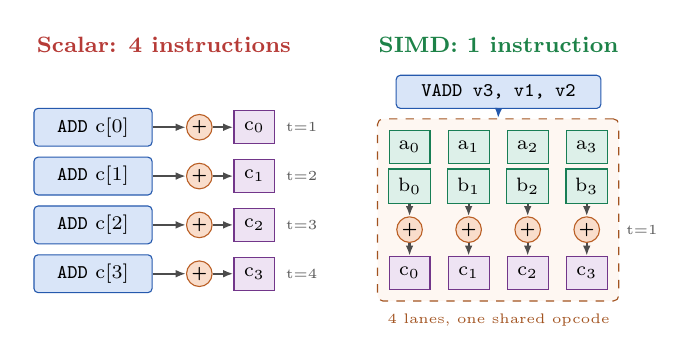
\begin{tikzpicture}[
    font=\scriptsize,
    ins/.style={draw=cFetch!80!black, fill=cFetch!18, rounded corners=1.5pt,
                minimum width=15mm, minimum height=4.2mm, align=center},
    el/.style={draw=cStore!80!black, fill=cStore!15, minimum width=5.2mm, minimum height=4.2mm},
    res/.style={draw=cWB!80!black, fill=cWB!15, minimum width=5.2mm, minimum height=4.2mm},
    alu/.style={draw=cComp!80!black, fill=cComp!25, circle, inner sep=0.6pt, font=\tiny\bfseries},
    arr/.style={-{Latex[length=1.3mm]}, thick, gray!60!black}
]
% ---------- scalar side ----------
\node[font=\footnotesize\bfseries, text=cFail!85!black] at (1.3,1.05) {Scalar: 4 instructions};
\foreach \i/\c in {0/1,1/2,2/3,3/4} {
  \node[ins] (si\i) at (0.4,-\i*0.62) {\texttt{ADD} c[\i]};
  \node[alu] (sa\i) at (1.75,-\i*0.62) {+};
  \node[res] (sr\i) at (2.45,-\i*0.62) {c\textsubscript{\i}};
  \draw[arr] (si\i) -- (sa\i);
  \draw[arr] (sa\i) -- (sr\i);
  \node[font=\tiny, text=gray!70!black] at (3.05,-\i*0.62) {t=\c};
}
% ---------- SIMD side ----------
\begin{scope}[xshift=4.3cm]
\node[font=\footnotesize\bfseries, text=cPass!75!black] at (1.25,1.05) {SIMD: 1 instruction};
\node[ins, minimum width=26mm] (vi) at (1.25,0.45) {\texttt{VADD v3, v1, v2}};
\foreach \i in {0,1,2,3} {
  \node[el]  (a\i) at (\i*0.75+0.12,-0.25) {a\textsubscript{\i}};
  \node[el]  (b\i) at (\i*0.75+0.12,-0.75) {b\textsubscript{\i}};
  \node[alu] (x\i) at (\i*0.75+0.12,-1.3) {+};
  \node[res] (r\i) at (\i*0.75+0.12,-1.85) {c\textsubscript{\i}};
  \draw[arr] (b\i) -- (x\i);
  \draw[arr] (x\i) -- (r\i);
}
\node[font=\tiny, text=gray!70!black, anchor=west] at (2.75,-1.3) {t=1};
\begin{scope}[on background layer]
\node[draw=cComp!70!black, dashed, rounded corners=2pt, fill=cComp!6,
      fit=(a0)(r3), inner sep=1.4mm] (lanes) {};
\end{scope}
\draw[arr, cFetch!80!black] (vi.south) -- (lanes.north);
\node[font=\tiny, text=cComp!70!black] at (1.25,-2.45) {4 lanes, one shared opcode};
\end{scope}
\end{tikzpicture}
\caption{Scalar versus SIMD execution of $c_i = a_i + b_i$ for four elements.
The scalar core fetches and decodes four instructions over four cycles; the
SIMD unit issues one \texttt{VADD} whose opcode drives four lane ALUs in a
single cycle.}
\label{fig:simdscalar}
\end{figure}

This project designs a small SIMD unit to study that trade-off directly in
hardware. The goals are to
(i) implement a vector datapath with four (and optionally eight) parallel lanes,
(ii) verify that every lane computes correctly and independently,
(iii) compare the same workload on scalar and SIMD configurations by cycle
count and throughput, and
(iv) measure the FPGA resource cost and maximum frequency of increasing the
number of lanes.
This report covers all four goals. Section~\ref{sec:lit} reviews related
work. Section~\ref{sec:solution} presents the architecture, the instruction set,
the verification methodology, the software tools and the measurement setup.
Section~\ref{sec:results} reports verification results, scalar-versus-SIMD
performance, hardware cost on an FPGA and the resulting time speedup.
Section~\ref{sec:contrib} lists individual contributions and
Section~\ref{sec:conclusion} concludes.
% -----------------------------------------------------------------------------
\section{Literature Review}
\label{sec:lit}

\subsection{Vector and SIMD architectures}
Flynn~\cite{flynn1972} classified computer organisations by their instruction
and data streams, with SIMD as the class in which one control unit drives many
processing elements. The CRAY-1~\cite{russell1978} made \emph{vector processing}
commercially successful: long vector registers were streamed through pipelined
functional units, so a single instruction could process up to 64 elements.
Hennessy and Patterson~\cite{hennessy2017} describe vector architectures, SIMD
instruction-set extensions and GPUs as three forms of data-level parallelism,
and identify lanes, vector registers and memory bandwidth as the main design
parameters.

\subsection{Packed SIMD extensions in general-purpose processors}
General-purpose processors adopted \emph{packed} SIMD, also called sub-word
parallelism, in which one wide register is split into several narrow lanes. HP's MAX-2~\cite{lee1996} and
Intel's MMX~\cite{peleg1996} added parallel 8/16/32-bit operations on 64-bit
registers for multimedia, including saturating arithmetic and parallel compares
that produce all-ones/all-zeros masks. Streaming SIMD Extensions~\cite{thakkar1999}
widened this to 128-bit registers with floating-point lanes. ARM's Advanced
SIMD (Neon)~\cite{armneon} provides comparable packed operations for embedded and
mobile processors, including vector-by-scalar forms that broadcast one operand to
all lanes. Our design follows this packed model: a vector is an $L\cdot W$-bit
word, lane $i$ occupies bits $[iW, iW+W-1]$, and compares produce lane masks in
the MMX style.

\subsection{Scalable vector ISAs}
The RISC-V Vector extension~\cite{riscvv2021} separates the instruction set from
the hardware vector length, so the same binary runs on implementations with
different numbers of lanes. It also defines vector-scalar (\texttt{.vx}) forms
and mask registers for predication. Kozyrakis and Patterson~\cite{kozyrakis2003}
argued that vector processors suit embedded systems because performance scales
by adding lanes, with modest growth in control complexity and energy. Our
\texttt{LANES} parameter follows the same idea at the hardware level: the
instruction set and control unit stay the same while the datapath width
changes.

\subsection{Vector processors on FPGAs}
Soft vector processors have been shown to accelerate data-parallel code on FPGAs.
Yu~\emph{et al.}~\cite{yu2008} attached a parameterised vector coprocessor to a
soft scalar CPU and reported speedups that grow with the number of lanes.
VESPA~\cite{yiannacouras2008} showed that the number of lanes, the vector length
and the memory interface can be tuned to trade FPGA area for performance. Both
note that speedup falls short of the lane count when scalar code, memory
accesses or control overhead dominate, as Amdahl's law~\cite{amdahl1967}
predicts. We measure this effect with scalar-versus-SIMD workloads on the
same RTL.

\subsection{Processor verification}
Directed tests cannot enumerate every instruction sequence of a processor.
Aharon~\emph{et al.}~\cite{aharon1995} generated random test programs and
compared the design against an architectural reference model, an approach
that found many bugs in industrial PowerPC processors. Mutation analysis,
introduced by DeMillo~\emph{et al.}~\cite{demillo1978}, measures a test
suite by planting small faults and counting how many it detects. We use both:
random programs against an independent instruction-set model, and planted RTL
faults to compare that method with the module testbenches.

\subsection{Positioning of this work}
Unlike the FPGA processors above, this project aims to be \emph{clear} rather
than as fast as possible. It uses a single-cycle datapath (CPI~$=1$), so cycle
counts can be checked by hand, and builds the scalar baseline from the same RTL,
so the only variable in the comparison is datapath width. Verification is treated
as a first-class result, using exhaustive, reference-model, random-program
and mutation testing, and all measurements use open-source
tools~\cite{shah2019} so that every number can be reproduced.
The design is written in Verilog~\cite{ieee1364} with SystemVerilog~\cite{ieee1800}
features used only in the testbenches.

\section{Proposed Solution}
\label{sec:solution}
% -----------------------------------------------------------------------------
\subsection{Architecture overview}
Fig.~\ref{fig:block} shows the complete unit. In each clock cycle the
instruction at the program counter is fetched and decoded by the vector control
unit. The register file supplies two source vectors. The lane multiplexer
selects operand~B as either the second vector or the scalar register broadcast
to all lanes. $L$ lane ALUs then compute in parallel under one shared opcode,
and the result combiner selects the write-back value from the ALU, the data
memory or the broadcast scalar. All state is updated on the next rising clock
edge, so every instruction completes in one cycle (CPI~$=1$). The design is
parameterised by \texttt{LANES} ($L$) and \texttt{WIDTH} ($W$). The vector
datapath modules use both parameters; each lane ALU uses only $W$, and the
decoder has a fixed ISA interface independent of $L$ and $W$. The scalar
baseline is the same RTL with $L=1$.
Supported project lane widths are $W=2,4,8,16$; wider configurations require
a revised reference model and separate validation.

\begin{figure*}[t]
\centering
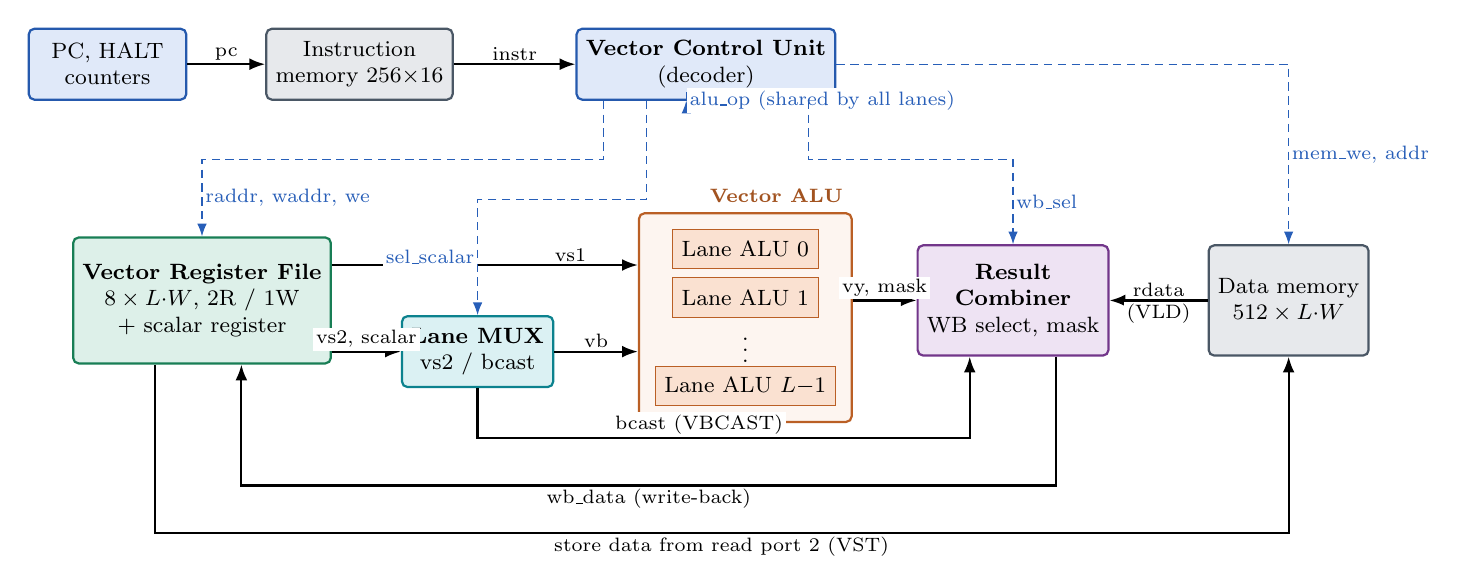
\begin{tikzpicture}[
    font=\footnotesize,
    blk/.style={draw, thick, rounded corners=2pt, align=center, minimum height=9mm,
                fill=white},
    fetch/.style={blk, draw=cFetch!80!black, fill=cFetch!15},
    stor/.style={blk, draw=cStore!80!black, fill=cStore!15},
    sel/.style={blk, draw=cSel!80!black, fill=cSel!15},
    wb/.style={blk, draw=cWB!80!black, fill=cWB!15},
    mem/.style={blk, draw=cMem!80!black, fill=cMem!15},
    lane/.style={draw=cComp!80!black, align=center, minimum width=17mm, minimum height=5mm,
                 fill=cComp!22},
    dat/.style={-{Latex[length=2mm]}, thick},
    ctl/.style={-{Latex[length=1.6mm]}, densely dashed, cFetch!85!black},
    lbl/.style={font=\scriptsize, fill=white, inner sep=1pt}
]
% ---- top row: fetch and decode ----
\node[fetch, minimum width=20mm] (pc)   at (0,0)    {PC, HALT\\counters};
\node[mem, minimum width=22mm] (imem) at (3.2,0)  {Instruction\\memory $256{\times}16$};
\node[fetch, minimum width=30mm] (ctrl) at (7.6,0)  {\textbf{Vector Control Unit}\\(decoder)};

% ---- datapath row ----
\node[stor, minimum width=26mm, minimum height=16mm] (rf) at (1.2,-3.0)
      {\textbf{Vector Register File}\\$8 \times L{\cdot}W$, 2R / 1W\\+ scalar register};
\node[sel, minimum width=16mm] (mux) at (4.7,-3.65) {\textbf{Lane MUX}\\vs2 / bcast};

\node[lane] (l0) at (8.1,-2.35) {Lane ALU 0};
\node[lane, below=1mm of l0] (l1) {Lane ALU 1};
\node[below=0mm of l1, inner sep=1pt] (ld) {$\vdots$};
\node[lane, below=0mm of ld] (l3) {Lane ALU $L{-}1$};
\begin{scope}[on background layer]
\node[draw=cComp!80!black, thick, rounded corners=2pt, fill=cComp!7, fit=(l0)(l3), inner sep=2mm,
      label={[font=\scriptsize, text=cComp!70!black, anchor=south east]north east:\textbf{Vector ALU}}] (valu) {};
\end{scope}

\node[wb, minimum width=22mm, minimum height=14mm] (rc) at (11.5,-3.0)
      {\textbf{Result}\\\textbf{Combiner}\\WB select, mask};
\node[mem, minimum width=20mm, minimum height=14mm] (dmem) at (15.0,-3.0)
      {Data memory\\$512 \times L{\cdot}W$};

% ---- data paths ----
\coordinate (vs1a) at ($(rf.east)+(0,0.45)$);
\coordinate (vs2a) at ($(rf.east)+(0,-0.65)$);
\coordinate (bcA)  at ($(rc.south)+(-0.55,0)$);
\coordinate (wbA)  at ($(rc.south)+(0.55,0)$);
\coordinate (wbB)  at ($(rf.south)+(0.5,0)$);
\coordinate (stA)  at ($(rf.south)+(-0.6,0)$);
\draw[dat] (pc) -- node[lbl, above]{pc} (imem);
\draw[dat] (imem) -- node[lbl, above]{instr} (ctrl);
\draw[dat] (vs1a) -- node[lbl, above, pos=0.78]{vs1} (vs1a -| valu.west);
\draw[dat] (vs2a) -- node[lbl, above]{vs2, scalar} (vs2a -| mux.west);
\draw[dat] (mux.east) -- node[lbl, above]{vb} (mux.east -| valu.west);
\draw[dat] (valu.east |- rc.west) -- node[lbl, above]{vy, mask} (rc.west);
\draw[dat] (dmem.west) -- node[lbl, above]{rdata} node[lbl, below]{(VLD)} (rc.east);
% broadcast scalar to the combiner (VBCAST)
\draw[dat] (mux.south) -- (mux.south |- 0,-4.75) -- node[lbl, above, pos=0.45]{bcast (VBCAST)}
           (bcA |- 0,-4.75) -- (bcA);
% write-back to the register file
\draw[dat] (wbA) -- (wbA |- 0,-5.35) -- node[lbl, below, pos=0.5]{wb\_data (write-back)}
           (wbB |- 0,-5.35) -- (wbB);
% store data from read port 2 to memory (VST)
\draw[dat] (stA) -- (stA |- 0,-5.95) -- node[lbl, below, pos=0.5]{store data from read port 2 (VST)}
           (dmem.south |- 0,-5.95) -- (dmem.south);

% ---- control signals ----
\draw[ctl] ($(ctrl.south)+(-1.3,0)$) -- ++(0,-0.75) -| node[lbl, pos=0.75, right]{raddr, waddr, we}
           (rf.north);
\draw[ctl] ($(ctrl.south)+(-0.75,0)$) -- ++(0,-1.25) -| node[lbl, pos=0.75, left]{sel\_scalar}
           (mux.north);
\draw[ctl] ($(ctrl.south)+(-0.25,0)$) -- node[lbl, pos=0.8, right]{alu\_op (shared by all lanes)}
           ($(ctrl.south)+(-0.25,0)$ |- valu.north);
\draw[ctl] ($(ctrl.south)+(1.3,0)$) -- ++(0,-0.75) -| node[lbl, pos=0.75, right]{wb\_sel}
           (rc.north);
\draw[ctl] (ctrl.east) -| node[lbl, pos=0.75, right]{mem\_we, addr} (dmem.north);
\end{tikzpicture}
\caption{Datapath of the SIMD vector unit, coloured by function: fetch and
control (blue), storage (green), operand select (teal), parallel compute
(orange), write-back (purple) and memories (grey). Solid arrows carry data,
dashed blue arrows carry control. The only signal shared by all lanes is the
decoded opcode (\texttt{alu\_op}).}
\label{fig:block}
\end{figure*}

\subsection{Top-level integration}
The module \texttt{simd\_top} connects the blocks of Fig.~\ref{fig:block} with
a 256-entry instruction memory, a 512-entry data memory in which one word holds
one full vector, an 8-bit program counter and a mask status register.
Three design choices make the top level robust and measurable:
\begin{itemize}
\item \textbf{Single point of write gating.} The decoder's register, scalar,
      memory and mask write enables are gated with
      $\neg\text{halted}\land\neg\text{rst}$, blocking instruction writes
      during reset and after \texttt{HALT}. Reset clears processor state and
      preserves both memories. The PC stays on \texttt{HALT}. Pre-filled
      \texttt{HALT} slots stop short programs; a full 256-slot image without
      \texttt{HALT} wraps and repeats. External sources must supply \texttt{HALT}.
\item \textbf{Performance counters.} \path{cycle_count} and
      \path{instr_count} count executed cycles and instructions (equal, since
      CPI~$=1$), and \path{lane_ops} adds $L$ for every vector ALU
      instruction. Throughput in element operations per cycle is therefore
      \path{lane_ops}/\path{cycle_count}.
\item \textbf{Debug read port.} An asynchronous read port on the data memory lets
      the testbench check results through the design's own interface. It also
      gives synthesis an observable path for stored datapath results. For resource
      estimation, a separate wrapper enables the optional external-instruction
      mode, so the default \texttt{HALT}-only instruction memory cannot make the
      datapath constant. Normal execution continues to fetch from instruction
      memory; instruction ROM is excluded from the synthesis estimate.
\end{itemize}
% -----------------------------------------------------------------------------
\subsection{Instruction set}
Instructions are 16 bits wide in three formats (Fig.~\ref{fig:fmt}). R-type
instructions include an $s$ bit that replaces \texttt{vs2} with the broadcast
scalar, so an operation such as ``add $k$ to every element'' needs only one
instruction, as in the vector-scalar forms of Neon and RISC-V~V. Table~\ref{tab:isa}
lists the opcodes; all sixteen 4-bit codes are used. All opcodes, field
positions and sizes are defined once in a shared header, \texttt{simd\_defs.vh},
which is itself checked by a testbench for unique opcodes and non-overlapping
fields.

\begin{figure}[t]
\centering
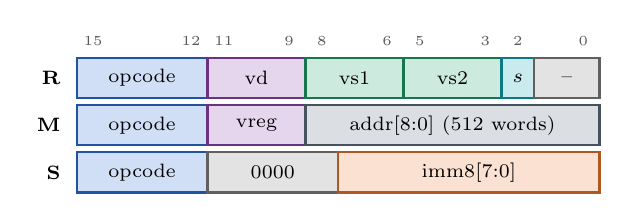
\begin{tikzpicture}[x=4.15mm, y=6mm, font=\scriptsize]
% field(row, msb, lsb, colour, text)
\newcommand{\fld}[5]{%
  \fill[#4!22] ({15-#2},{-#1}) rectangle ({16-#3},{-#1-0.85});
  \draw[#4!75!black, thick] ({15-#2},{-#1}) rectangle ({16-#3},{-#1-0.85});
  \node at ({(31-#2-#3)/2},{-#1-0.425}) {#5};}
% bit numbers
\foreach \b in {15,12,11,9,8,6,5,3,2,0}
  \node[font=\tiny, text=gray!70!black] at ({15.5-\b},0.35) {\b};
% R-type
\node[anchor=east, font=\scriptsize\bfseries] at (-0.2,-0.425) {R};
\fld{0}{15}{12}{cFetch}{opcode}
\fld{0}{11}{9}{cWB}{vd}
\fld{0}{8}{6}{cStore}{vs1}
\fld{0}{5}{3}{cStore}{vs2}
\fld{0}{2}{2}{cSel}{$s$}
\fld{0}{1}{0}{gray}{--}
% M-type
\node[anchor=east, font=\scriptsize\bfseries] at (-0.2,-1.425) {M};
\fld{1}{15}{12}{cFetch}{opcode}
\fld{1}{11}{9}{cWB}{vreg}
\fld{1}{8}{0}{cMem}{addr[8:0] (512 words)}
% S-type
\node[anchor=east, font=\scriptsize\bfseries] at (-0.2,-2.425) {S};
\fld{2}{15}{12}{cFetch}{opcode}
\fld{2}{11}{8}{gray}{0000}
\fld{2}{7}{0}{cComp}{imm8[7:0]}
\end{tikzpicture}
\caption{16-bit instruction formats. R-type: vector ALU operations and
\texttt{VBCAST}; $s=1$ replaces \texttt{vs2} with the broadcast scalar.
M-type: \texttt{VLD}/\texttt{VST}. S-type: \texttt{SLI}. Grey fields are zero.}
\label{fig:fmt}
\end{figure}

\begin{table}[t]
\centering
\caption{Instruction set (per lane $i$; $B = s\,?\,\text{scalar} : \text{vs2}$)}
\label{tab:isa}
\footnotesize
\setlength{\tabcolsep}{4pt}
\begin{tabular}{@{}lll@{}}
\toprule
Opcode & Mnemonic & Operation \\
\midrule
0001/0010 & VADD/VSUB & $vd_i = vs1_i \pm B_i$ (mod $2^W$) \\
0011--0101 & VAND/VOR/VXOR & $vd_i = vs1_i \circ B_i$ (bitwise) \\
0110 & VCMPEQ & $vd_i = (vs1_i = B_i)$ ? all-ones : 0 \\
0111 & VCMPLT & signed $vs1_i < B_i$ ? all-ones : 0 \\
1000/1001 & VSLL/VSRL & $vs1_i \ll / \gg B_i[\log_2 W-1:0]$ \\
1010 & VMUL & low $W$ bits of $vs1_i \times B_i$ \\
1011 & SLI & scalar $=$ imm8 (zero-extended) \\
1100/1101 & VLD/VST & vreg $\leftrightarrow$ DMEM[addr] \\
1110 & VBCAST & $vd_i =$ scalar \\
0000/1111 & NOP/HALT & -- \\
\bottomrule
\end{tabular}
\end{table}

\subsection{Vector control unit and result combiner}
\paragraph{Vector control unit} A purely combinational decoder that produces the
ALU opcode, register addresses, write enables, write-back select and the
\texttt{halt} and \texttt{mask\_we} flags. Register addresses are taken straight
from the instruction fields; only the enables depend on the opcode. For
\texttt{VST} the second read port is redirected to the store register, so store
data always leaves the register file through port~2. Every instruction has at
most one data destination among the vector registers, scalar register and data
memory (\texttt{rf\_we + mem\_we + s\_we} $\leq 1$). Compare instructions
additionally update mask status through \texttt{mask\_we}.

\paragraph{Result combiner} Selects the write-back value from the ALU, the data
memory (\texttt{VLD}) or the broadcast scalar (\texttt{VBCAST}); the reserved
select code writes zero rather than an unknown value. It also reduces the
per-lane compare mask to \emph{any}, \emph{all} and population-count outputs,
the hardware counterparts of mask-test instructions in commercial SIMD
extensions.
% -----------------------------------------------------------------------------
\subsection{Lane ALU and vector ALU}
\paragraph{Lane ALU} A combinational $W$-bit ALU implementing the ten vector
operations. Every path assigns default outputs first, so no latches are
inferred, and non-ALU opcodes produce zero. Arithmetic wraps modulo $2^W$.
\texttt{VCMPLT} uses a signed (two's-complement) comparison, so
\texttt{0xFF}~($-1$) is less than \texttt{0x01}. The shift amount is the low
$\log_2 W$ bits of operand~B, as in x86 and RISC-V, which is why $W$ must be a
power of two. Compares drive a \texttt{flag} output and write all-ones or
all-zeros to the lane, so the result can be used directly as a bit mask.

\paragraph{Vector ALU} A \texttt{generate} loop creates $L$ lane ALUs, each
connected to its own $W$-bit slice $[iW, iW+W-1]$ of the operands and the
result. The opcode is the only signal shared between lanes, so carries,
borrows and shifted bits never cross a lane boundary. This is the property that
separates a SIMD datapath from a single wide ALU: one $32$-bit adder computes
$\texttt{0xFFFFFFFF} + \texttt{0x01010101} = \texttt{0x01010100}$, whereas four
8-bit lanes correctly produce \texttt{0x00000000}. Each lane's compare flag forms
bit $i$ of the lane mask.
% -----------------------------------------------------------------------------
\subsection{Vector register file and lane multiplexer}
\paragraph{Vector register file} Eight $L\cdot W$-bit registers with two
combinational read ports and one write port that updates on the rising clock
edge, plus a $W$-bit scalar register with its own write port. A read during a
write returns the old value until the clock edge. This is the correct behaviour
for a single-cycle datapath: \texttt{VADD v1,v1,v2} reads the old \texttt{v1}
and its result replaces \texttt{v1} at the end of the cycle, so no forwarding
logic is needed. A synchronous reset clears every register. The register file
is the largest flip-flop cost in the core and grows linearly with $L$
($8 \times 32 = 256$ flip-flops at $L=4$).

\paragraph{Lane multiplexer} Selects operand~B as \texttt{vs2} or
$\{L\{\text{scalar}\}\}$. The broadcast itself is only wiring, since every lane's
input is connected to the same $W$ scalar bits; the hardware cost is one 2:1
multiplexer per bit. The replicated scalar is also exported so that
\texttt{VBCAST} reuses it through the result combiner.
% -----------------------------------------------------------------------------
\subsection{Verification methodology}
Each module has a self-checking testbench. The ALU reference uses integer
modulo arithmetic and explicit two's-complement conversion to reduce shared
implementation errors. At $W=8$, all $2^{16}$ operand pairs are tested for each
of the ten lane-ALU operations; the decoder tests all $2^{16}$ instruction
words. Other tests combine directed cases with random vectors. Whole-processor
tests compare all memory words, registers, scalar, mask, PC and counters with
an instruction-set model.

Guards require every ALU opcode, 4{,}096 words per decoder opcode, and nonempty
register-file, MUX and combiner test sections. Each lane's compare flag must be
seen low and high, and all four write-back selections exercised. Six
incomplete-stimulus probes are rejected.

\texttt{make verify\_matrix} saves twelve configuration runs in
\path{results/verification_matrix.txt}. \texttt{make mutation\_tests}
saves passing baselines and 23 detected faults in \path{results/mutations.txt},
plus coverage probes in \path{results/coverage_guards.txt}. Logs include tool
versions, commands, source hashes and exact mutations. Build errors, timeouts
and survivors fail verification.
Fig.~\ref{fig:verif} shows the flow and Table~\ref{tab:ver} summarises the
results.

\begin{figure}[t]
\centering
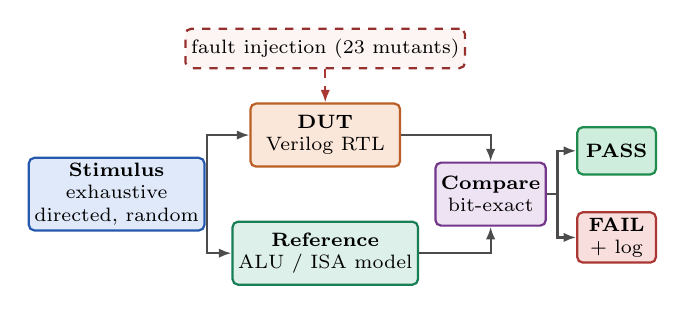
\begin{tikzpicture}[
    font=\scriptsize,
    box/.style={draw, thick, rounded corners=2pt, align=center, inner sep=2pt,
                minimum height=8mm},
    arr/.style={-{Latex[length=1.6mm]}, thick, gray!60!black}
]
\node[box, draw=cFetch!80!black, fill=cFetch!15, minimum width=15mm] (stim) at (0,0)
     {\textbf{Stimulus}\\exhaustive\\directed, random};
\node[box, draw=cComp!80!black, fill=cComp!18, minimum width=19mm] (dut) at (2.65,0.75)
     {\textbf{DUT}\\Verilog RTL};
\node[box, draw=cStore!80!black, fill=cStore!15, minimum width=19mm] (ref) at (2.65,-0.75)
     {\textbf{Reference}\\ALU / ISA model};
\node[box, draw=cWB!80!black, fill=cWB!15, minimum width=12mm] (cmp) at (4.75,0)
     {\textbf{Compare}\\bit-exact};
\node[box, draw=cPass!80!black, fill=cPass!22, minimum width=10mm, minimum height=6mm]
     (pass) at (6.35,0.55) {\textbf{PASS}};
\node[box, draw=cFail!80!black, fill=cFail!18, minimum width=10mm, minimum height=6mm]
     (fail) at (6.35,-0.55) {\textbf{FAIL}\\+ log};
\node[box, draw=cFail!70!black, dashed, fill=cFail!6, minimum height=5mm]
     (inj) at (2.65,1.85) {fault injection (23 mutants)};
\draw[arr] (stim.east) -- (1.15,0) |- (dut.west);
\draw[arr] (stim.east) -- (1.15,0) |- (ref.west);
\draw[arr] (dut.east) -| (cmp.north);
\draw[arr] (ref.east) -| (cmp.south);
\draw[arr] (cmp.east) -- (5.6,0) |- (pass.west);
\draw[arr] (cmp.east) -- (5.6,0) |- (fail.west);
\draw[arr, dashed, cFail!80!black] (inj) -- (dut);
\end{tikzpicture}
\caption{Self-checking verification flow used by every testbench. The same
stimulus drives the RTL and an independent reference model; any mismatch is
logged as a failure. All 23 seeded RTL faults are detected.}
\label{fig:verif}
\end{figure}

\begin{table}[t]
\centering
\caption{Verification results ($L=4$, $W=8$)}
\label{tab:ver}
\footnotesize
\begin{tabular}{@{}llr@{}}
\toprule
Module & Method & Checks \\
\midrule
Lane ALU        & exhaustive $\times$ 10 ops      & 656{,}650 \\
Vector ALU      & isolation, walking lane, masks  & 51{,}277 \\
Register file   & shadow model, read-during-write & 15{,}248 \\
Lane MUX        & all 256 scalars broadcast       & 12{,}772 \\
Result combiner & distinct sources, all masks     & 19{,}216 \\
Control unit    & all 65{,}536 instructions       & 65{,}536 \\
Top level       & 8 scenarios and boundary checks & 5{,}274 \\
\midrule
\multicolumn{2}{@{}l}{Total (incl.\ spec and smoke tests), all pass} & 826{,}122 \\
\multicolumn{2}{@{}l}{Injected faults detected} & 23 / 23 \\
\bottomrule
\end{tabular}
\end{table}

P1--P8 produce nine final-state comparisons: P7 is checked at \texttt{HALT} and
50 cycles later. P6 checks PC wrap over 258 \texttt{NOP} cycles. P8 resets on a
pending \texttt{VST}, checking all 512 memory words and cleared processor state.
The reference normalizes operands modulo $2^W$. The 826{,}122 total applies to
$L=4$, $W=8$. CPI~$=1$: \texttt{VLD, VLD, VADD, VST, HALT} takes five cycles
and four element operations; the 44-instruction all-operations program takes
44 cycles and 80 element operations.
Fig.~\ref{fig:wave} shows the simulated waveform of the vector-add program,
loaded from \texttt{programs/add.hex}: during the \texttt{VADD} cycle the four
lane results ($17, 18, 19, 20$) are all produced together and written back on
a single clock edge.

\begin{figure*}[t]
\centering
% Generated by scripts/vcd_to_tikz.py from sim/run_programs.vcd - do not edit by hand
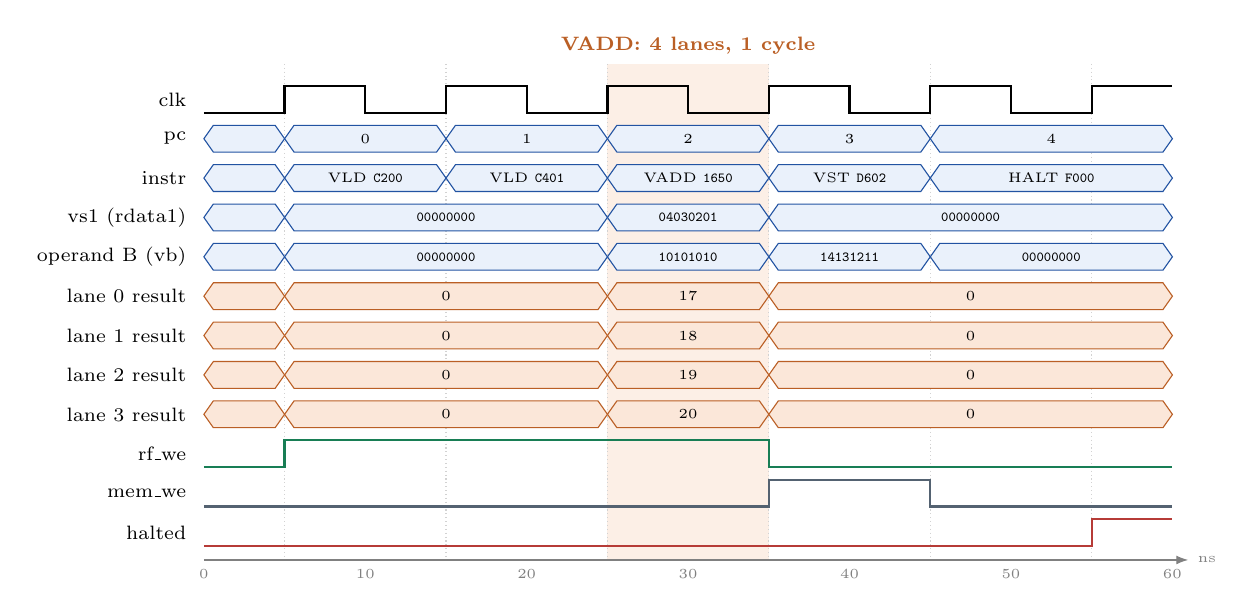
\begin{tikzpicture}[font=\scriptsize,
  bus/.style={draw=cFetch!75!black, fill=cFetch!10, thin},
  lanebus/.style={draw=cComp!80!black, fill=cComp!18, thin},
  val/.style={font=\tiny, inner sep=0}]
\fill[cComp!12] (5.125,0.45) rectangle (7.175,-5.85);
\node[font=\scriptsize\bfseries, text=cComp!80!black, anchor=south] at (6.150,0.45) {VADD: 4 lanes, 1 cycle};
\draw[gray!35, densely dotted] (1.025,0.45) -- (1.025,-5.85);
\draw[gray!35, densely dotted] (3.075,0.45) -- (3.075,-5.85);
\draw[gray!35, densely dotted] (5.125,0.45) -- (5.125,-5.85);
\draw[gray!35, densely dotted] (7.175,0.45) -- (7.175,-5.85);
\draw[gray!35, densely dotted] (9.225,0.45) -- (9.225,-5.85);
\draw[gray!35, densely dotted] (11.275,0.45) -- (11.275,-5.85);
\node[anchor=east, font=\scriptsize] at (-0.1,0.00) {clk};
\draw[thick, black] (0.000,0.00-0.17) -- (1.025,0.00-0.17) -- (1.025,0.00+0.17) -- (2.050,0.00+0.17) -- (2.050,0.00-0.17) -- (3.075,0.00-0.17) -- (3.075,0.00+0.17) -- (4.100,0.00+0.17) -- (4.100,0.00-0.17) -- (5.125,0.00-0.17) -- (5.125,0.00+0.17) -- (6.150,0.00+0.17) -- (6.150,0.00-0.17) -- (7.175,0.00-0.17) -- (7.175,0.00+0.17) -- (8.200,0.00+0.17) -- (8.200,0.00-0.17) -- (9.225,0.00-0.17) -- (9.225,0.00+0.17) -- (10.250,0.00+0.17) -- (10.250,0.00-0.17) -- (11.275,0.00-0.17) -- (11.275,0.00+0.17) -- (12.300,0.00+0.17);
\node[anchor=east, font=\scriptsize] at (-0.1,-0.50) {pc};
\draw[bus] (0.000,-0.50) -- (0.000+0.12,-0.50+0.17) -- (1.025-0.12,-0.50+0.17) -- (1.025,-0.50) -- (1.025-0.12,-0.50-0.17) -- (0.000+0.12,-0.50-0.17) -- cycle;
\draw[bus] (1.025,-0.50) -- (1.025+0.12,-0.50+0.17) -- (3.075-0.12,-0.50+0.17) -- (3.075,-0.50) -- (3.075-0.12,-0.50-0.17) -- (1.025+0.12,-0.50-0.17) -- cycle;
\node[val] at (2.050,-0.50) {0};
\draw[bus] (3.075,-0.50) -- (3.075+0.12,-0.50+0.17) -- (5.125-0.12,-0.50+0.17) -- (5.125,-0.50) -- (5.125-0.12,-0.50-0.17) -- (3.075+0.12,-0.50-0.17) -- cycle;
\node[val] at (4.100,-0.50) {1};
\draw[bus] (5.125,-0.50) -- (5.125+0.12,-0.50+0.17) -- (7.175-0.12,-0.50+0.17) -- (7.175,-0.50) -- (7.175-0.12,-0.50-0.17) -- (5.125+0.12,-0.50-0.17) -- cycle;
\node[val] at (6.150,-0.50) {2};
\draw[bus] (7.175,-0.50) -- (7.175+0.12,-0.50+0.17) -- (9.225-0.12,-0.50+0.17) -- (9.225,-0.50) -- (9.225-0.12,-0.50-0.17) -- (7.175+0.12,-0.50-0.17) -- cycle;
\node[val] at (8.200,-0.50) {3};
\draw[bus] (9.225,-0.50) -- (9.225+0.12,-0.50+0.17) -- (12.300-0.12,-0.50+0.17) -- (12.300,-0.50) -- (12.300-0.12,-0.50-0.17) -- (9.225+0.12,-0.50-0.17) -- cycle;
\node[val] at (10.762,-0.50) {4};
\node[anchor=east, font=\scriptsize] at (-0.1,-1.00) {instr};
\draw[bus] (0.000,-1.00) -- (0.000+0.12,-1.00+0.17) -- (1.025-0.12,-1.00+0.17) -- (1.025,-1.00) -- (1.025-0.12,-1.00-0.17) -- (0.000+0.12,-1.00-0.17) -- cycle;
\draw[bus] (1.025,-1.00) -- (1.025+0.12,-1.00+0.17) -- (3.075-0.12,-1.00+0.17) -- (3.075,-1.00) -- (3.075-0.12,-1.00-0.17) -- (1.025+0.12,-1.00-0.17) -- cycle;
\node[val] at (2.050,-1.00) {VLD \texttt{C200}};
\draw[bus] (3.075,-1.00) -- (3.075+0.12,-1.00+0.17) -- (5.125-0.12,-1.00+0.17) -- (5.125,-1.00) -- (5.125-0.12,-1.00-0.17) -- (3.075+0.12,-1.00-0.17) -- cycle;
\node[val] at (4.100,-1.00) {VLD \texttt{C401}};
\draw[bus] (5.125,-1.00) -- (5.125+0.12,-1.00+0.17) -- (7.175-0.12,-1.00+0.17) -- (7.175,-1.00) -- (7.175-0.12,-1.00-0.17) -- (5.125+0.12,-1.00-0.17) -- cycle;
\node[val] at (6.150,-1.00) {VADD \texttt{1650}};
\draw[bus] (7.175,-1.00) -- (7.175+0.12,-1.00+0.17) -- (9.225-0.12,-1.00+0.17) -- (9.225,-1.00) -- (9.225-0.12,-1.00-0.17) -- (7.175+0.12,-1.00-0.17) -- cycle;
\node[val] at (8.200,-1.00) {VST \texttt{D602}};
\draw[bus] (9.225,-1.00) -- (9.225+0.12,-1.00+0.17) -- (12.300-0.12,-1.00+0.17) -- (12.300,-1.00) -- (12.300-0.12,-1.00-0.17) -- (9.225+0.12,-1.00-0.17) -- cycle;
\node[val] at (10.762,-1.00) {HALT \texttt{F000}};
\node[anchor=east, font=\scriptsize] at (-0.1,-1.50) {vs1 (rdata1)};
\draw[bus] (0.000,-1.50) -- (0.000+0.12,-1.50+0.17) -- (1.025-0.12,-1.50+0.17) -- (1.025,-1.50) -- (1.025-0.12,-1.50-0.17) -- (0.000+0.12,-1.50-0.17) -- cycle;
\draw[bus] (1.025,-1.50) -- (1.025+0.12,-1.50+0.17) -- (5.125-0.12,-1.50+0.17) -- (5.125,-1.50) -- (5.125-0.12,-1.50-0.17) -- (1.025+0.12,-1.50-0.17) -- cycle;
\node[val] at (3.075,-1.50) {\texttt{00000000}};
\draw[bus] (5.125,-1.50) -- (5.125+0.12,-1.50+0.17) -- (7.175-0.12,-1.50+0.17) -- (7.175,-1.50) -- (7.175-0.12,-1.50-0.17) -- (5.125+0.12,-1.50-0.17) -- cycle;
\node[val] at (6.150,-1.50) {\texttt{04030201}};
\draw[bus] (7.175,-1.50) -- (7.175+0.12,-1.50+0.17) -- (12.300-0.12,-1.50+0.17) -- (12.300,-1.50) -- (12.300-0.12,-1.50-0.17) -- (7.175+0.12,-1.50-0.17) -- cycle;
\node[val] at (9.737,-1.50) {\texttt{00000000}};
\node[anchor=east, font=\scriptsize] at (-0.1,-2.00) {operand B (vb)};
\draw[bus] (0.000,-2.00) -- (0.000+0.12,-2.00+0.17) -- (1.025-0.12,-2.00+0.17) -- (1.025,-2.00) -- (1.025-0.12,-2.00-0.17) -- (0.000+0.12,-2.00-0.17) -- cycle;
\draw[bus] (1.025,-2.00) -- (1.025+0.12,-2.00+0.17) -- (5.125-0.12,-2.00+0.17) -- (5.125,-2.00) -- (5.125-0.12,-2.00-0.17) -- (1.025+0.12,-2.00-0.17) -- cycle;
\node[val] at (3.075,-2.00) {\texttt{00000000}};
\draw[bus] (5.125,-2.00) -- (5.125+0.12,-2.00+0.17) -- (7.175-0.12,-2.00+0.17) -- (7.175,-2.00) -- (7.175-0.12,-2.00-0.17) -- (5.125+0.12,-2.00-0.17) -- cycle;
\node[val] at (6.150,-2.00) {\texttt{10101010}};
\draw[bus] (7.175,-2.00) -- (7.175+0.12,-2.00+0.17) -- (9.225-0.12,-2.00+0.17) -- (9.225,-2.00) -- (9.225-0.12,-2.00-0.17) -- (7.175+0.12,-2.00-0.17) -- cycle;
\node[val] at (8.200,-2.00) {\texttt{14131211}};
\draw[bus] (9.225,-2.00) -- (9.225+0.12,-2.00+0.17) -- (12.300-0.12,-2.00+0.17) -- (12.300,-2.00) -- (12.300-0.12,-2.00-0.17) -- (9.225+0.12,-2.00-0.17) -- cycle;
\node[val] at (10.762,-2.00) {\texttt{00000000}};
\node[anchor=east, font=\scriptsize] at (-0.1,-2.50) {lane 0 result};
\draw[lanebus] (0.000,-2.50) -- (0.000+0.12,-2.50+0.17) -- (1.025-0.12,-2.50+0.17) -- (1.025,-2.50) -- (1.025-0.12,-2.50-0.17) -- (0.000+0.12,-2.50-0.17) -- cycle;
\draw[lanebus] (1.025,-2.50) -- (1.025+0.12,-2.50+0.17) -- (5.125-0.12,-2.50+0.17) -- (5.125,-2.50) -- (5.125-0.12,-2.50-0.17) -- (1.025+0.12,-2.50-0.17) -- cycle;
\node[val] at (3.075,-2.50) {0};
\draw[lanebus] (5.125,-2.50) -- (5.125+0.12,-2.50+0.17) -- (7.175-0.12,-2.50+0.17) -- (7.175,-2.50) -- (7.175-0.12,-2.50-0.17) -- (5.125+0.12,-2.50-0.17) -- cycle;
\node[val] at (6.150,-2.50) {17};
\draw[lanebus] (7.175,-2.50) -- (7.175+0.12,-2.50+0.17) -- (12.300-0.12,-2.50+0.17) -- (12.300,-2.50) -- (12.300-0.12,-2.50-0.17) -- (7.175+0.12,-2.50-0.17) -- cycle;
\node[val] at (9.737,-2.50) {0};
\node[anchor=east, font=\scriptsize] at (-0.1,-3.00) {lane 1 result};
\draw[lanebus] (0.000,-3.00) -- (0.000+0.12,-3.00+0.17) -- (1.025-0.12,-3.00+0.17) -- (1.025,-3.00) -- (1.025-0.12,-3.00-0.17) -- (0.000+0.12,-3.00-0.17) -- cycle;
\draw[lanebus] (1.025,-3.00) -- (1.025+0.12,-3.00+0.17) -- (5.125-0.12,-3.00+0.17) -- (5.125,-3.00) -- (5.125-0.12,-3.00-0.17) -- (1.025+0.12,-3.00-0.17) -- cycle;
\node[val] at (3.075,-3.00) {0};
\draw[lanebus] (5.125,-3.00) -- (5.125+0.12,-3.00+0.17) -- (7.175-0.12,-3.00+0.17) -- (7.175,-3.00) -- (7.175-0.12,-3.00-0.17) -- (5.125+0.12,-3.00-0.17) -- cycle;
\node[val] at (6.150,-3.00) {18};
\draw[lanebus] (7.175,-3.00) -- (7.175+0.12,-3.00+0.17) -- (12.300-0.12,-3.00+0.17) -- (12.300,-3.00) -- (12.300-0.12,-3.00-0.17) -- (7.175+0.12,-3.00-0.17) -- cycle;
\node[val] at (9.737,-3.00) {0};
\node[anchor=east, font=\scriptsize] at (-0.1,-3.50) {lane 2 result};
\draw[lanebus] (0.000,-3.50) -- (0.000+0.12,-3.50+0.17) -- (1.025-0.12,-3.50+0.17) -- (1.025,-3.50) -- (1.025-0.12,-3.50-0.17) -- (0.000+0.12,-3.50-0.17) -- cycle;
\draw[lanebus] (1.025,-3.50) -- (1.025+0.12,-3.50+0.17) -- (5.125-0.12,-3.50+0.17) -- (5.125,-3.50) -- (5.125-0.12,-3.50-0.17) -- (1.025+0.12,-3.50-0.17) -- cycle;
\node[val] at (3.075,-3.50) {0};
\draw[lanebus] (5.125,-3.50) -- (5.125+0.12,-3.50+0.17) -- (7.175-0.12,-3.50+0.17) -- (7.175,-3.50) -- (7.175-0.12,-3.50-0.17) -- (5.125+0.12,-3.50-0.17) -- cycle;
\node[val] at (6.150,-3.50) {19};
\draw[lanebus] (7.175,-3.50) -- (7.175+0.12,-3.50+0.17) -- (12.300-0.12,-3.50+0.17) -- (12.300,-3.50) -- (12.300-0.12,-3.50-0.17) -- (7.175+0.12,-3.50-0.17) -- cycle;
\node[val] at (9.737,-3.50) {0};
\node[anchor=east, font=\scriptsize] at (-0.1,-4.00) {lane 3 result};
\draw[lanebus] (0.000,-4.00) -- (0.000+0.12,-4.00+0.17) -- (1.025-0.12,-4.00+0.17) -- (1.025,-4.00) -- (1.025-0.12,-4.00-0.17) -- (0.000+0.12,-4.00-0.17) -- cycle;
\draw[lanebus] (1.025,-4.00) -- (1.025+0.12,-4.00+0.17) -- (5.125-0.12,-4.00+0.17) -- (5.125,-4.00) -- (5.125-0.12,-4.00-0.17) -- (1.025+0.12,-4.00-0.17) -- cycle;
\node[val] at (3.075,-4.00) {0};
\draw[lanebus] (5.125,-4.00) -- (5.125+0.12,-4.00+0.17) -- (7.175-0.12,-4.00+0.17) -- (7.175,-4.00) -- (7.175-0.12,-4.00-0.17) -- (5.125+0.12,-4.00-0.17) -- cycle;
\node[val] at (6.150,-4.00) {20};
\draw[lanebus] (7.175,-4.00) -- (7.175+0.12,-4.00+0.17) -- (12.300-0.12,-4.00+0.17) -- (12.300,-4.00) -- (12.300-0.12,-4.00-0.17) -- (7.175+0.12,-4.00-0.17) -- cycle;
\node[val] at (9.737,-4.00) {0};
\node[anchor=east, font=\scriptsize] at (-0.1,-4.50) {rf\_we};
\draw[thick, cStore!80!black] (0.000,-4.50-0.17) -- (1.025,-4.50-0.17) -- (1.025,-4.50+0.17) -- (7.175,-4.50+0.17) -- (7.175,-4.50-0.17) -- (12.300,-4.50-0.17);
\node[anchor=east, font=\scriptsize] at (-0.1,-5.00) {mem\_we};
\draw[thick, cMem!90!black] (0.000,-5.00-0.17) -- (1.025,-5.00-0.17) -- (1.025,-5.00-0.17) -- (7.175,-5.00-0.17) -- (7.175,-5.00+0.17) -- (9.225,-5.00+0.17) -- (9.225,-5.00-0.17) -- (12.300,-5.00-0.17);
\node[anchor=east, font=\scriptsize] at (-0.1,-5.50) {halted};
\draw[thick, cFail!85!black] (0.000,-5.50-0.17) -- (1.025,-5.50-0.17) -- (1.025,-5.50-0.17) -- (11.275,-5.50-0.17) -- (11.275,-5.50+0.17) -- (12.300,-5.50+0.17);
\draw[-{Latex[length=1.5mm]}, gray] (0,-5.85) -- (12.300+0.2,-5.85) node[right, font=\tiny] {ns};
\node[font=\tiny, gray, below] at (0.000,-5.85) {0};
\node[font=\tiny, gray, below] at (2.050,-5.85) {10};
\node[font=\tiny, gray, below] at (4.100,-5.85) {20};
\node[font=\tiny, gray, below] at (6.150,-5.85) {30};
\node[font=\tiny, gray, below] at (8.200,-5.85) {40};
\node[font=\tiny, gray, below] at (10.250,-5.85) {50};
\node[font=\tiny, gray, below] at (12.300,-5.85) {60};
\end{tikzpicture}

\caption{Simulation waveform of the vector-add program
(\texttt{VLD, VLD, VADD, VST, HALT}) with $L=4$, $W=8$, drawn directly from the
Icarus Verilog VCD by \texttt{scripts/vcd\_to\_tikz.py}. The ALU output is split
into its four 8-bit lanes: in the highlighted \texttt{VADD} cycle every lane
computes $vs1_i + vs2_i$ simultaneously, and \texttt{rf\_we} commits the whole
vector at the next rising edge. The program halts after exactly five cycles.}
\label{fig:wave}
\end{figure*}

% Fig. 6 is defined here (not in Section V) so it floats onto the same page as
% Fig. 5 instead of being stranded alone on the last page.
\begin{figure*}[t]
\centering
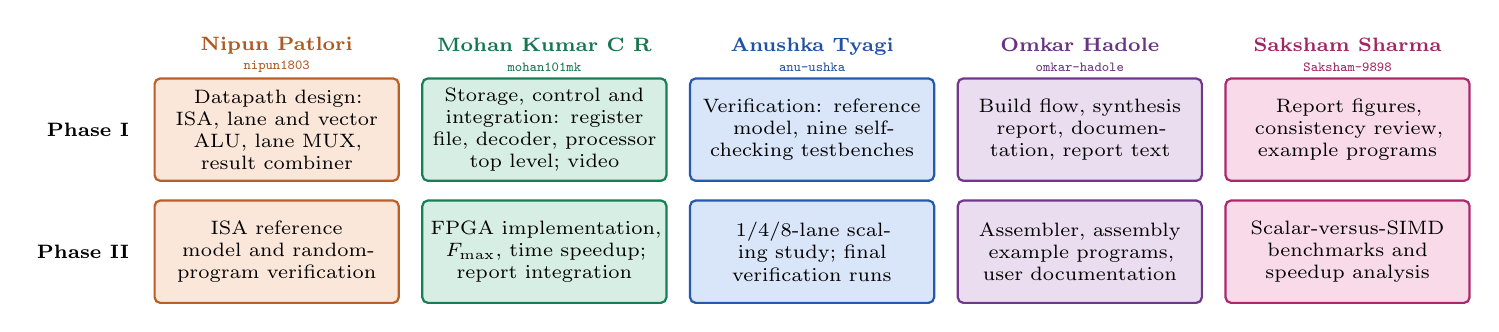
\begin{tikzpicture}[
    font=\scriptsize,
    role/.style={draw=#1!80!black, fill=#1!18, thick, rounded corners=2pt,
                 minimum width=31mm, text width=29mm, minimum height=13mm, align=center, inner sep=2pt},
    head/.style={font=\scriptsize\bfseries, text=#1!75!black, align=center},
    row/.style={font=\scriptsize\bfseries, anchor=east, align=right}
]
\foreach \x/\c/\n/\u in {0/cNip/Nipun Patlori/nipun1803, 1/cMoh/Mohan Kumar C R/mohan101mk,
                         2/cAnu/Anushka Tyagi/anu-ushka, 3/cOmk/Omkar Hadole/omkar-hadole,
                         4/cSak/Saksham Sharma/Saksham-9898}
  \node[head=\c] at (\x*3.4, 0.95) {\n\\[-1pt]{\normalfont\ttfamily\tiny \u}};
\node[row] at (-1.75, 0) {Phase I};
\node[role=cNip] at (0.0, 0) {Datapath design: ISA, lane and vector ALU, lane MUX, result combiner};
\node[role=cMoh] at (3.4, 0) {Storage, control and integration: register file, decoder, processor top level; video};
\node[role=cAnu] at (6.8, 0) {Verification: reference model, nine self-checking testbenches};
\node[role=cOmk] at (10.2, 0) {Build flow, synthesis report, documentation, report text};
\node[role=cSak] at (13.6, 0) {Report figures, consistency review, example programs};
\node[row] at (-1.75, -1.55) {Phase II};
\node[role=cNip] at (0.0, -1.55) {ISA reference model and random-program verification};
\node[role=cMoh] at (3.4, -1.55) {FPGA implementation, $F_{\max}$, time speedup; report integration};
\node[role=cAnu] at (6.8, -1.55) {1/4/8-lane scaling study; final verification runs};
\node[role=cOmk] at (10.2, -1.55) {Assembler, assembly example programs, user documentation};
\node[role=cSak] at (13.6, -1.55) {Scalar-versus-SIMD benchmarks and speedup analysis};
\end{tikzpicture}
\caption{Role of each team member in Phase~I and Phase~II.}
\label{fig:team}
\end{figure*}

\subsection{Software tools}
\textbf{Assembler.} \path{scripts/lfasm.py} translates assembly into the
hex files loaded by the instruction and data memories. It reads opcodes and
field positions from \texttt{simd\_defs.vh}, the header the RTL includes, so
the two cannot diverge. Directives place data words lane by lane
(\texttt{.vec}), and errors are reported with file and line. Its tests check
the encoding table of the instruction-set document and all $2^{16}$
instruction words through disassembly and reassembly.

\textbf{Independent ISA model.} \path{scripts/lfmodel.py} is a Python model
written from the instruction-set document, not from the RTL or the Verilog
model in \texttt{tb\_simd\_top}. Its field positions are hard-coded rather
than read from the shared header, so an error in the header appears as a
mismatch instead of being copied.

\textbf{Program runner.} \path{tb/prog_runner.v} runs any number of programs
on one compiled build: it resets, reloads both memories, runs to \texttt{HALT}
or a cycle limit and dumps the final state. A comparison covers
eight status values (cycles, instructions, lane operations, mask, scalar, PC,
\texttt{HALT} and steps), the eight vector registers and all 512 data words;
unknown (\texttt{X}) bits count as mismatches.

\subsection{Random-program verification}
For each of the twelve builds, a seeded generator produces programs of up to
255 instructions over all sixteen opcodes. It biases operands towards edge values
(0, 1, all ones, the sign bit), sets reserved bits at random, draws addresses
from a small pool so that stores are re-read and overwritten, and inserts
occasional mid-program \texttt{HALT}s; every 40th program is a full 256-word
image without \texttt{HALT}, which wraps the program counter. The model
records functional-coverage goals (each opcode, each ALU opcode with the
scalar operand, each lane's compare true and false, carries, borrows,
multiply overflow, shift amounts $\ge W$, signed compares across zero,
store-to-load hazards, back-to-back dependencies, ignored bits and PC
wrap-around). Goals that depend on the build, such as one compare goal per
lane, exist only where they apply, so a build has between \RandGoalsMin{} and
\RandGoalsMax{} goals, and it fails if any applicable goal is missed.

\subsection{Benchmark workloads}
Table~\ref{tab:work} lists the four kernels. A generator writes each kernel in
assembly for a lane count $L$ and $N$ elements; the same data is used for every
$L$. Because the instruction set has no branches, every loop is unrolled, and
with CPI~$=1$ the cycle count follows directly from the program length. Each
run is checked three ways: the output arrays against plain Python, the full
final state against the ISA model, and the cycle count against the formula.
W2 uses the fact that a true compare writes $-1$ to its lane: subtracting the
compare result adds one to that lane's count, giving three instructions per
vector. It leaves one partial count per lane, because the ISA has no
cross-lane (horizontal) add. We therefore also give an \emph{estimate} for W2
that charges $L-1$ extra cycles for summing the lanes; those cycles are
assumed, not executed. Speedup and time speedup are
\begin{equation}
S(L) = \frac{\text{cycles}(1)}{\text{cycles}(L)},\qquad
S_t(L) = S(L)\,\frac{F_{\max}(L)}{F_{\max}(1)} .
\end{equation}

\begin{table}[t]
\centering
\caption{Benchmark kernels ($N$ elements, $L$ lanes)}
\label{tab:work}
\footnotesize
\setlength{\tabcolsep}{4pt}
\begin{tabular}{@{}lll@{}}
\toprule
Kernel & Instructions per vector & Cycles \\
\midrule
W1 $C=A+B$ & \texttt{VLD, VLD, VADD, VST} & $4N/L+1$ \\
W2 count$(A<T)$ & \texttt{VLD, VCMPLT s, VSUB} & $3N/L+3$ \\
W3 $(A\wedge M)\vee B$ & \texttt{VLD}$\times$3\texttt{, VAND, VOR, VST} & $6N/L+1$ \\
W4 $aX+b$ & \texttt{VLD, VMUL s, VADD, VST} & $4N/L+4$ \\
\bottomrule
\end{tabular}
\end{table}

\subsection{Synthesis and FPGA flow}
Generic synthesis uses the \texttt{simd\_synth\_top} wrapper and
Yosys~\cite{yosys} with variable instruction inputs; it includes the datapath,
the 512-word data memory, PC and counters, and excludes instruction ROM.
For the FPGA, Yosys \texttt{synth\_ecp5} and nextpnr-ecp5~\cite{shah2019}
implement the design on a Lattice LFE5U-85F~\cite{ecp5ds} (CABGA381, speed
grade~6). The wrapper \texttt{fpga\_top} feeds the instruction and debug
address from a free-running 32-bit LFSR and XOR-folds every output into one
registered pin. Nothing can be optimised away, only three pins are needed, and
because inputs and output are registered, $F_{\max}$ is set by the processor's
own register-to-register paths. Each build is placed and routed with three
seeds; we report the median $F_{\max}$.

% -----------------------------------------------------------------------------
\section{Results and Discussion}
\label{sec:results}

\subsection{Functional verification}
The module testbenches pass in all \MatrixConfigs{} configurations of
$L=1,4,8$ and $W=2,4,8,16$, with \ModuleChecks{} checks at $L=4$, $W=8$
(Table~\ref{tab:ver}), and detect all \UnitMutDetected{} planted RTL faults.
Random-program verification ran \RandPerBuild{} programs on each of the
\RandBuilds{} builds: \RandPrograms{} programs, \RandInstr{} executed
instructions and \RandValues{} compared state values, with no mismatch. Every
applicable coverage goal was hit on every build (\RandGoalsMin{} to
\RandGoalsMax{} goals per build).

Running only the random programs against the same \MutTotal{} faults shows how
the two methods differ. \RandMutDetected{} faults change the final state and
are detected. One (a register-file read port that forwards a pending write)
forms a combinational loop through the ALU, and the simulation never finishes.
The remaining \RandMutMissed{} alter only internal signals that never reach
architectural state: the \emph{any}-lane flag, the mask population count, and
the reserved write-back select, which the decoder never produces. No program
can expose them, but the module testbenches do. Each method catches faults
the other cannot reach, so both are needed.

\subsection{Scalar versus SIMD performance}
Table~\ref{tab:bench} and Fig.~\ref{fig:speedup} give the measured cycle counts
for $N=32$; every run matches its predicted cycle count exactly and passes all
three checks. W3 comes closest to the ideal speedup: it does the most work per vector
and has only one fixed instruction (\texttt{HALT}), reaching
\SpeedupThreeEight$\times$ at $L=8$. W2 and W4 carry three or four
setup and final instructions that do not shrink with $L$, so their speedup
saturates sooner (\SpeedupFourEight$\times$ at $L=8$), as Amdahl's
law~\cite{amdahl1967} predicts. The effect grows for short arrays: at $N=8$
the 8-lane W2 reaches only \SpeedupTwoEightSmall$\times$. Charging an
estimated $L-1$ cycles for the cross-lane sum, which this ISA cannot perform,
would lower W2 at $L=8$ from \SpeedupTwoEight$\times$ to about
\SpeedupTwoEightRed$\times$. This shows why commercial SIMD instruction sets
include horizontal-add or reduction instructions.

\begin{table}[t]
\centering
\caption{Cycles and speedup, $N=32$, $W=8$}
\label{tab:bench}
\footnotesize
\setlength{\tabcolsep}{3.2pt}
\begin{tabular}{@{}lrrrrrl@{}}
\toprule
 & \multicolumn{3}{c}{Cycles} & \multicolumn{2}{c}{Speedup} & Elements \\
\cmidrule(lr){2-4}\cmidrule(lr){5-6}
Kernel & $L{=}1$ & $L{=}4$ & $L{=}8$ & $L{=}4$ & $L{=}8$ & per cycle \\
\midrule
\BenchRows
\bottomrule
\multicolumn{7}{@{}l}{\scriptsize $^\ddagger$ estimate: $L-1$ assumed cycles for the per-lane sum (not executed)}
\end{tabular}
\end{table}

\begin{figure}[t]
\centering
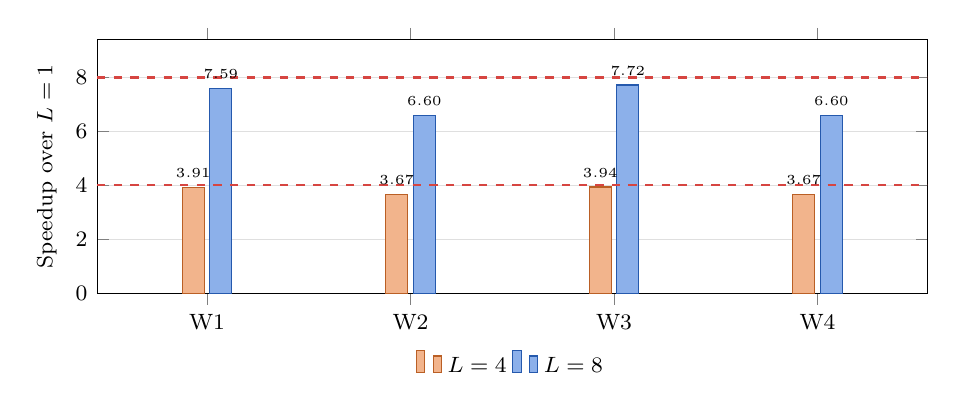
\begin{tikzpicture}
\begin{axis}[
    ybar, bar width=8pt, width=\columnwidth, height=4.8cm,
    symbolic x coords={W1,W2,W3,W4}, xtick=data,
    ymin=0, ymax=9.4, ytick={0,2,4,6,8}, ylabel={Speedup over $L=1$},
    ylabel style={font=\footnotesize}, tick label style={font=\footnotesize},
    legend style={font=\footnotesize, at={(0.5,-0.2)}, anchor=north, legend columns=2, draw=none},
    nodes near coords, nodes near coords style={font=\tiny, /pgf/number format/.cd, fixed, precision=2, fixed zerofill},
    enlarge x limits=0.18, ymajorgrids, grid style={gray!25}]
\addplot[fill=cComp!55, draw=cComp!80!black] coordinates {\SpeedupFourCoords};
\addplot[fill=cFetch!55, draw=cFetch!80!black] coordinates {\SpeedupEightCoords};
\legend{$L=4$, $L=8$}
\draw[cFail, dashed, thick] (rel axis cs:0,4/9.4) -- (rel axis cs:1,4/9.4);
\draw[cFail, dashed, thick] (rel axis cs:0,8/9.4) -- (rel axis cs:1,8/9.4);
\end{axis}
\end{tikzpicture}
\caption{Measured cycle speedup of the 4- and 8-lane builds over the scalar
build for $N=32$. Dashed lines mark the ideal speedup $S=L$.}
\label{fig:speedup}
\end{figure}

\subsection{Hardware cost}
Table~\ref{tab:synth} gives generic cell counts. The SIMD core grows
\CoreGrowthFour$\times$ from one to four lanes and \CoreGrowthEight$\times$
to eight, almost exactly in proportion to $L$, while the decoder stays at 25
cells. The data memory dominates the total because generic synthesis builds
it from flip-flops (\GenericFlopsFour{} at $L=4$).

On the ECP5 (Table~\ref{tab:fpga}) the picture changes. Yosys maps the data
memory to distributed LUT RAM, with one copy per read port, so only
\FlopsFour{} flip-flops remain at $L=4$. Each lane uses one DSP multiplier
for \texttt{VMUL}, block RAM is not used because the memory has asynchronous
reads, and the 8-lane build occupies 16\% of the device's logic cells. Core LUTs
grow in proportion to $L$; the data memory, PC and counters remain the
largest single block.

\begin{table}[t]
\centering
\caption{Generic synthesis cells (Yosys), $W=8$}
\label{tab:synth}
\footnotesize
\begin{tabular}{@{}lrrr@{}}
\toprule
Block & $L{=}1$ & $L{=}4$ & $L{=}8$ \\
\midrule
\SynthRows
\bottomrule
\end{tabular}
\end{table}

\begin{table}[t]
\centering
\caption{Lattice ECP5-85F implementation, $W=8$}
\label{tab:fpga}
\footnotesize
\begin{tabular}{@{}lrrr@{}}
\toprule
 & $L{=}1$ & $L{=}4$ & $L{=}8$ \\
\midrule
\FpgaRows
\bottomrule
\end{tabular}
\end{table}

\subsection{Clock frequency and time speedup}
The median $F_{\max}$ falls from \FmaxOne{} to \FmaxFour{} and \FmaxEight{}~MHz.
In every build the critical path is the load: it starts at the instruction's
address bits, passes through the 512-entry data-memory read multiplexer and
ends at a vector-register flip-flop. Logic delay stays near 7--7.5~ns; the
path grows from \PathOne{} to \PathEight{}~ns mainly through routing, because
wider vectors spread the memory and register file across more of the chip.
Table~\ref{tab:eff} combines cycles and clock: the 8-lane build loses
\ClockLossEight\% of its clock but still adds two arrays
\EffOneEight$\times$ faster in time, using \CombRatioEight$\times$ the logic
cells. The cross-lane sum is the weak point: with the estimated lane-sum
cycles, W2 gains only about 3.9$\times$ in time.

\begin{table}[t]
\centering
\caption{Execution time and time speedup $S_t$, $N=32$}
\label{tab:eff}
\footnotesize
\setlength{\tabcolsep}{4pt}
\begin{tabular}{@{}lrrrr@{}}
\toprule
 & \multicolumn{2}{c}{Time (ns)} & \multicolumn{2}{c}{$S_t$} \\
\cmidrule(lr){2-3}\cmidrule(lr){4-5}
Kernel & $L{=}1$ & $L{=}8$ & $L{=}4$ & $L{=}8$ \\
\midrule
\EffRows
\bottomrule
\multicolumn{5}{@{}l}{\scriptsize $^\dagger$ estimate: $+(L-1)$ assumed lane-sum cycles}
\end{tabular}
\end{table}

\subsection{Limitations}
The measurements have known limits. Programs are straight-line because the
ISA has no branches, and the 256-entry instruction memory caps the scalar
kernels at 42 (W3) to 63 (W1) elements. The FPGA wrapper drives instructions from an LFSR,
so it measures resources and timing, not a running program; functional
behaviour is verified in simulation. Instruction ROM is excluded from all
resource counts. Timing comes from the open-source nextpnr timing model at
speed grade~6, not from a vendor tool or hardware. Finally, the single-cycle
design puts the memory read and the ALU in one clock period, which is the main
reason for the modest clock frequency.

% -----------------------------------------------------------------------------
\section{Individual Contributions}
\label{sec:contrib}
In Phase~I the work was divided by layer of the design: datapath, storage and
control, verification, build and documentation, and figures. In Phase~II it
was divided by study: software tools, random verification, performance,
scaling and FPGA implementation. Fig.~\ref{fig:team} summarises each member's
role in both phases. A recorded video demonstration of the Phase~I prototype is
available at \url{https://drive.google.com/drive/folders/17inRVThPM6PJx6WKdC6LPiTfmpqH07jN}.

\begin{itemize}
\item \textbf{Nipun Patlori} (\texttt{nipun1803}) -- \emph{Datapath designer
      and random-verification lead.} Phase~I: defined the instruction
      set's opcodes and instruction formats and designed the datapath: the
      lane ALU, the vector ALU that replicates it across all lanes, the lane
      multiplexer that broadcasts the scalar operand, and the result combiner
      with its compare-mask summary; also produced the simulation waveform
      figure and wrote the Phase~I conclusion. Phase~II: built the
      independent instruction-set reference model and the random-program
      verification: a program runner for the processor, a seeded random
      program generator with functional-coverage goals, the comparison of
      twelve thousand random programs against the model in all twelve
      configurations, and the experiment that scores random testing against
      the planted faults.
\item \textbf{Mohan Kumar C R} (\texttt{mohan101mk}) -- \emph{Storage, control
      and integration designer; FPGA implementation lead.} Phase~I:
      designed the vector register file and scalar register, the instruction
      decoder, and the complete single-cycle processor that joins all blocks
      with the instruction and data memories, program counter, halt logic,
      performance counters and debug port; also recorded the prototype video.
      Phase~II: implemented the processor on a Lattice ECP5 FPGA with the
      open-source flow, designed the measurement wrapper, measured logic,
      memory, DSP use and maximum frequency for one, four and eight lanes,
      analysed the critical path, and derived the time speedup; also
      integrated the final report, with result tables generated directly from
      the evidence, and wrote the abstract, introduction and conclusion.
\item \textbf{Anushka Tyagi} (\texttt{anu-ushka}) -- \emph{Verification
      engineer and scaling-study lead.} Phase~I: built the complete
      module-level verification suite: the shared testbench infrastructure, the
      independent ALU reference model and nine self-checking testbenches,
      including exhaustive tests of the lane ALU and decoder, lane-isolation
      tests and a whole-processor test against an instruction-set model.
      Phase~II: carried out the scaling study, synthesising the design for
      one, four and eight lanes and analysing how the cost of every block grows
      with the lane count; re-ran the full verification matrix and the
      planted-fault campaign on the final design, and wrote the functional
      verification and hardware-cost results.
\item \textbf{Omkar Hadole} (\texttt{omkar-hadole}) -- \emph{Build,
      documentation and software-tools lead.} Phase~I: set up the project
      structure and the build and simulation flow, produced the first synthesis
      report, wrote the project documentation, and wrote the Phase~I report text
      and references. Phase~II: developed the assembler, which translates
      assembly programs into memory images, places data lane by lane, reports
      errors by line, disassembles machine code and is tested on every
      possible instruction word; rewrote the example programs in assembly
      and updated the user documentation for the new tools.
\item \textbf{Saksham Sharma} (\texttt{Saksham-9898}) -- \emph{Figures, review
      and performance-evaluation lead.} Phase~I: drew the report figures
      (scalar versus SIMD execution, the colour-coded datapath, instruction
      formats, verification flow and the team map), reviewed the README,
      report and repository for consistency, and wrote the runnable example
      programs with their demo check. Phase~II: ran the scalar-versus-SIMD
      evaluation: four benchmark kernels (array addition, threshold counting,
      bitwise masking and scale-and-offset) generated for one, four and eight
      lanes and checked against expected results, the reference model and the
      predicted cycle counts; analysed the speedup, including the
      fixed-overhead and cross-lane reduction limits, and produced the speedup
      chart and the performance results.
\end{itemize}

% -----------------------------------------------------------------------------
\section{Conclusion}
\label{sec:conclusion}
This work delivers a parameterised SIMD vector processing unit in
synthesisable Verilog, together with the tools to program, verify and measure
it. The design passes \ModuleChecks{} module-level checks, exhaustive tests of
the lane ALU and decoder, and \RandPrograms{} random programs compared with an
independent instruction-set model in all \MatrixConfigs{} configurations;
module tests and random programs together expose every planted fault that
can affect behaviour. Because the scalar baseline is the same RTL with one lane,
the comparison isolates the effect of datapath width. Eight lanes need up to
\SpeedupThreeEight$\times$ fewer cycles, logic grows almost in proportion to
the lane count, and the clock drops by \ClockLossEight\%. The net result is a
\EffOneEight$\times$ faster array addition on an ECP5 FPGA. Speedup is limited by fixed
setup instructions and by the missing cross-lane reduction.

Natural extensions are a pipelined datapath, which would separate the memory
read from the ALU and raise the clock; branch instructions for loops;
a horizontal-add instruction for reductions; and synchronous memory reads, so
the data memory can use block RAM.

\bibliographystyle{IEEEtran}
\bibliography{references}

\end{document}
